\documentclass[11pt,a4paper]{article}
\usepackage[margin=1in]{geometry}
\usepackage{amsmath,amssymb}
\usepackage{booktabs}
\usepackage{graphicx}
\usepackage{hyperref}
\usepackage[numbers]{natbib}
\usepackage{xcolor}
\usepackage{siunitx}
\usepackage{tikz}
\usetikzlibrary{arrows.meta,positioning,shapes.geometric}
\usepackage{float}
\usepackage{enumitem}
\usepackage{caption}
\usepackage{longtable}
\usepackage{multicol}
\usepackage{array}
\usepackage{colortbl}

\hypersetup{colorlinks=true, linkcolor=blue!60!black, citecolor=green!50!black, urlcolor=blue!70!black}

\title{\textbf{Techno-Economic Assessment of\\Natural Olivine Valorization}\\[8pt]
\large CO\textsubscript{2} Sequestration, H\textsubscript{2} Production, and Iron Recovery\\via Direct Carbonation and Serpentinization}

\author{Separation-Agents Automated Valorization Pipeline\\
\texttt{sep\_agents v0.3}}

\date{March 2026}

\begin{document}
\maketitle

%──────────────────────────────────────────────────────────────────────
\begin{abstract}
This report presents a techno-economic analysis of valorizing natural olivine ore (85\,vol\% forsterite Mg\textsubscript{2}SiO\textsubscript{4}, 15\,vol\% fayalite Fe\textsubscript{2}SiO\textsubscript{4}) at a throughput of \SI{100}{t/d}.
Three value streams were identified: CO\textsubscript{2} sequestration via direct carbonation of forsterite (\$25.80/t revenue), magnetite concentrate from serpentinization (\$12.19/t), and green H\textsubscript{2} production (\$3.54/t).
Four process topologies were evaluated using a Generalized Disjunctive Programming (GDP) superstructure framework with IDAES-PSE simulation and JAX-based techno-economic modeling.
The optimal topology (Config-2: heat recovery only, with magnetic separation) yields products of 0.13\,kg H\textsubscript{2}/t, 3.0\,kg CO\textsubscript{2} sequestered/t, and 15.2\,kg Fe\textsubscript{3}O\textsubscript{4}/t ore.
At current commodity prices and \SI{100}{t/d} scale, the project is uneconomic (net $-$\SI{200}{USD/t}) with labor dominating OPEX at 86\%.
Economy of scale (\SI{1000}{t/d}+), higher CO\textsubscript{2} credit prices (\$100+/t), and co-location with existing mineral processing operations represent the primary pathways to viability.
\end{abstract}

\tableofcontents
\newpage

%──────────────────────────────────────────────────────────────────────
\section{Introduction and Opportunity}

Olivine is one of the most abundant minerals in the Earth's upper mantle, with massive surface deposits found in Norway, Pakistan, Australia, and the western United States.
Natural olivine is a solid-solution series between the Mg-endmember forsterite (Mg\textsubscript{2}SiO\textsubscript{4}) and the Fe-endmember fayalite (Fe\textsubscript{2}SiO\textsubscript{4}).
Its high Mg and Fe content creates multiple simultaneous valorization opportunities:

\begin{enumerate}[noitemsep]
  \item \textbf{CO\textsubscript{2} mineral carbonation:} Forsterite reacts directly with CO\textsubscript{2} to form thermodynamically stable MgCO\textsubscript{3}, permanently sequestering carbon and generating carbon credits.
  \item \textbf{H\textsubscript{2} production:} Fayalite undergoes aqueous serpentinization at elevated temperature and pressure, producing molecular hydrogen.
  \item \textbf{Iron recovery:} Serpentinization produces magnetite (Fe\textsubscript{3}O\textsubscript{4}), recoverable via low-intensity magnetic separation (LIMS).
  \item \textbf{Construction aggregate:} Residual SiO\textsubscript{2} from both reactions is suitable for aggregate or filler applications.
\end{enumerate}

This study evaluates the techno-economic feasibility of a combined serpentinization--carbonation process treating \SI{100}{t/d} of natural olivine ore.
Speciation was not required: all value streams involve stoichiometric solid-state or gas--solid reactions amenable to direct engineering models.

%──────────────────────────────────────────────────────────────────────
\section{Raw Material Composition}

\subsection{Mineralogy}

The feed consists of natural olivine with 85\,vol\% forsterite and 15\,vol\% fayalite.
Using mineral densities ($\rho_{\text{Fo}}$ = 3.27\,g/cm\textsuperscript{3}, $\rho_{\text{Fa}}$ = 4.39\,g/cm\textsuperscript{3}), the weight fractions are computed as 80.8\,wt\% forsterite and 19.2\,wt\% fayalite.

\begin{table}[H]
\centering
\caption{Olivine Feed Composition}
\label{tab:composition}
\begin{tabular}{lcccl}
\toprule
\textbf{Mineral} & \textbf{vol\%} & \textbf{wt\%} & \textbf{mol/kg} & \textbf{Role} \\
\midrule
Forsterite (Mg\textsubscript{2}SiO\textsubscript{4}) & 85.0 & 80.8 & 5.746 & CO\textsubscript{2} carbonation feedstock \\
Fayalite (Fe\textsubscript{2}SiO\textsubscript{4})   & 15.0 & 19.2 & 0.940 & H\textsubscript{2} production, Fe recovery \\
\bottomrule
\end{tabular}
\end{table}

\subsection{Oxide Basis}

\begin{table}[H]
\centering
\caption{Bulk Oxide Composition}
\label{tab:oxide}
\begin{tabular}{lcc}
\toprule
\textbf{Oxide} & \textbf{wt\%} & \textbf{Role} \\
\midrule
MgO                         & 46.3 & CO\textsubscript{2} carbonation \\
SiO\textsubscript{2}        & 40.2 & Aggregate co-product \\
FeO                         & 13.5 & H\textsubscript{2} production, Fe recovery \\
\midrule
\textit{Total}              & 100.0 & \\
\bottomrule
\end{tabular}
\end{table}

%──────────────────────────────────────────────────────────────────────
\section{Process Description}

The process uses a \textbf{series configuration}: olivine first undergoes serpentinization (consuming Fe\textsubscript{2}SiO\textsubscript{4}), then the Mg\textsubscript{2}SiO\textsubscript{4}-rich residue proceeds to direct carbonation with added CO\textsubscript{2}.

\subsection{Process Flow Diagram}

\begin{figure}[H]
\centering
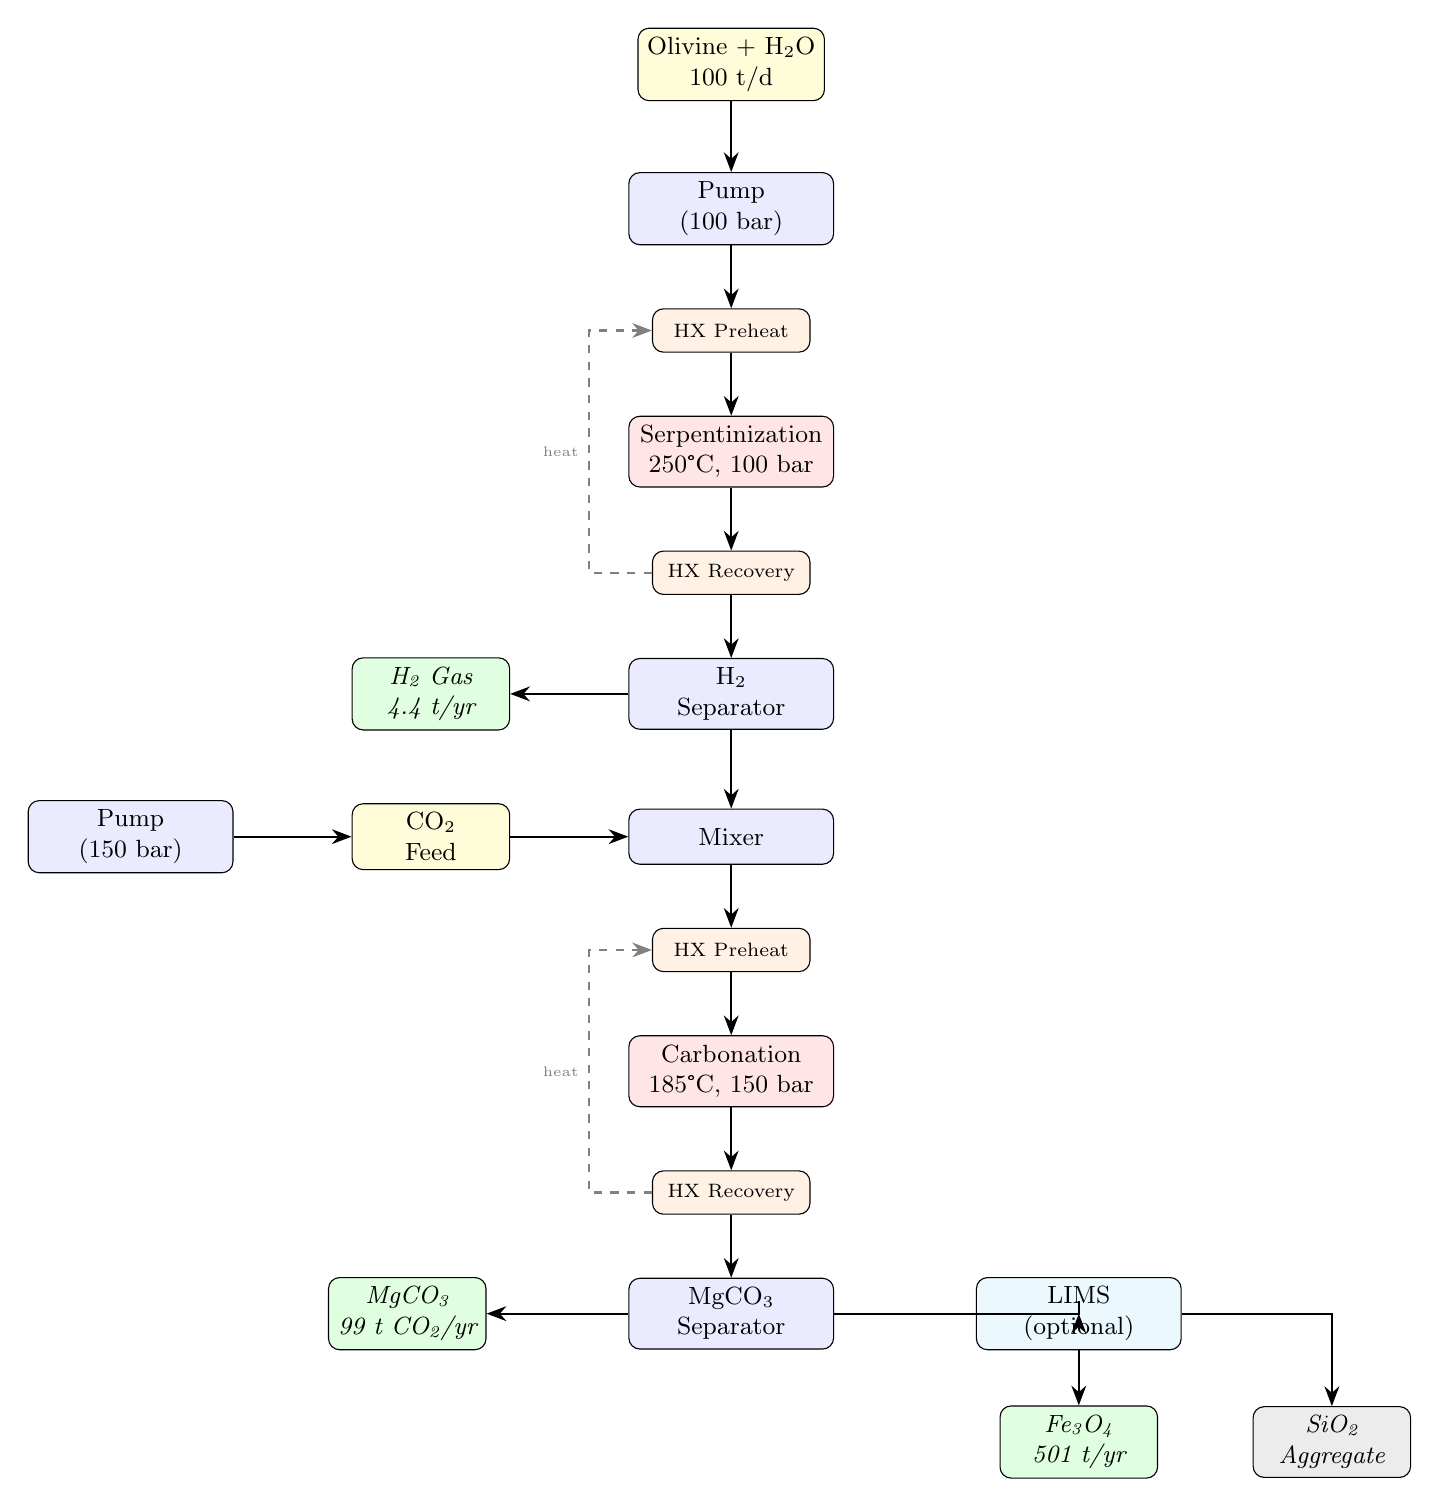
\begin{tikzpicture}[
  node distance=1.4cm and 2.0cm,
  unit/.style={rectangle, draw, rounded corners, minimum width=2.6cm,
               minimum height=0.7cm, align=center, fill=blue!8, font=\small},
  hx/.style={rectangle, draw, rounded corners, minimum width=2.0cm,
             minimum height=0.55cm, align=center, fill=orange!10, font=\scriptsize},
  product/.style={rectangle, draw, rounded corners, minimum width=2.0cm,
                  minimum height=0.5cm, align=center, fill=green!12,
                  font=\small\itshape},
  feed/.style={rectangle, draw, rounded corners, minimum width=2.0cm,
               minimum height=0.5cm, align=center, fill=yellow!15,
               font=\small},
  stream/.style={-{Stealth[length=2.5mm]}, thick},
]
  % -- Column 1: Serpentinization Train --
  \node[feed] (olivine) {Olivine + H\textsubscript{2}O\\100 t/d};
  \node[unit, below=0.9cm of olivine] (pump1) {Pump\\(100 bar)};
  \node[hx, below=0.8cm of pump1] (hx1) {HX Preheat};
  \node[unit, below=0.8cm of hx1, fill=red!10] (serp) {Serpentinization\\250\textdegree C, 100 bar};
  \node[hx, below=0.8cm of serp] (hx3) {HX Recovery};
  \node[unit, below=0.8cm of hx3] (sep1) {H\textsubscript{2}\\Separator};

  % Products from serp
  \node[product, left=1.5cm of sep1] (h2) {H\textsubscript{2} Gas\\4.4 t/yr};

  % -- Mixer + Column 2: Carbonation Train --
  \node[unit, below=1.0cm of sep1] (mixer) {Mixer};
  \node[feed, left=1.5cm of mixer] (co2) {CO\textsubscript{2}\\Feed};
  \node[unit, left=1.5cm of co2] (pump2) {Pump\\(150 bar)};

  \node[hx, below=0.8cm of mixer] (hx2) {HX Preheat};
  \node[unit, below=0.8cm of hx2, fill=red!10] (carb) {Carbonation\\185\textdegree C, 150 bar};
  \node[hx, below=0.8cm of carb] (hx4) {HX Recovery};
  \node[unit, below=0.8cm of hx4] (sep2) {MgCO\textsubscript{3}\\Separator};

  % Products from carb
  \node[product, left=1.8cm of sep2] (mgco3) {MgCO\textsubscript{3}\\99 t CO\textsubscript{2}/yr};

  % Optional LIMS
  \node[unit, right=1.8cm of sep2, fill=cyan!8] (lims) {LIMS\\(optional)};
  \node[product, below=0.7cm of lims] (fe3o4) {Fe\textsubscript{3}O\textsubscript{4}\\501 t/yr};
  \node[product, right=1.2cm of fe3o4, fill=gray!15] (agg) {SiO\textsubscript{2}\\Aggregate};

  % Connections
  \draw[stream] (olivine) -- (pump1);
  \draw[stream] (pump1) -- (hx1);
  \draw[stream] (hx1) -- (serp);
  \draw[stream] (serp) -- (hx3);
  \draw[stream] (hx3) -- (sep1);
  \draw[stream] (sep1) -- (h2);
  \draw[stream] (sep1) -- (mixer);
  \draw[stream] (co2) -- (mixer);
  \draw[stream] (pump2) -- (co2);
  \draw[stream] (mixer) -- (hx2);
  \draw[stream] (hx2) -- (carb);
  \draw[stream] (carb) -- (hx4);
  \draw[stream] (hx4) -- (sep2);
  \draw[stream] (sep2) -- (mgco3);
  \draw[stream] (sep2.east) -| (lims);
  \draw[stream] (lims) -- (fe3o4);
  \draw[stream] (lims.east) -| (agg);

  % Heat recovery arrows
  \draw[stream, dashed, gray] (hx3.west) -- +(-0.8,0) |- node[pos=0.25, left, font=\tiny, gray] {heat} (hx1.west);
  \draw[stream, dashed, gray] (hx4.west) -- +(-0.8,0) |- node[pos=0.25, left, font=\tiny, gray] {heat} (hx2.west);

\end{tikzpicture}
\caption{Process flow diagram for olivine valorization --- series configuration with optional LIMS for Fe\textsubscript{3}O\textsubscript{4} recovery.}
\label{fig:pfd}
\end{figure}

\subsection{Key Reactions}

\paragraph{Serpentinization (H\textsubscript{2} production):}
\begin{equation}
  3\text{Fe}_2\text{SiO}_4 + 2\text{H}_2\text{O} \longrightarrow
  2\text{Fe}_3\text{O}_4 + 3\text{SiO}_2 + 2\text{H}_2 \uparrow
  \label{eq:serp}
\end{equation}
Conditions: \SI{250}{\celsius}, \SI{100}{bar}; 70\% conversion of Fe\textsubscript{2}SiO\textsubscript{4}.

\paragraph{Direct carbonation of forsterite:}
\begin{equation}
  \text{Mg}_2\text{SiO}_4 + 2\text{CO}_2 \longrightarrow
  2\text{MgCO}_3 + \text{SiO}_2
  \label{eq:carb}
\end{equation}
Conditions: \SI{185}{\celsius}, \SI{150}{bar}; 80\% conversion of Mg\textsubscript{2}SiO\textsubscript{4}.

%──────────────────────────────────────────────────────────────────────
\section{Modeling Approach}

\begin{table}[H]
\centering
\caption{Two-Tier Modeling Hierarchy (No Aqueous Speciation Required)}
\label{tab:modeling}
\begin{tabular}{p{3cm}p{4cm}p{5cm}}
\toprule
\textbf{Tier} & \textbf{Tool} & \textbf{Application} \\
\midrule
Process Simulation & IDAES-PSE / Pyomo & Stoichiometric reactor mass balances, GDP superstructure optimization \\
Economic & JAX TEA + autodiff & Itemized CAPEX/OPEX, EAC, cost sensitivity \\
\bottomrule
\end{tabular}
\end{table}

Aqueous equilibrium speciation (Reaktoro) was \textbf{not required} for this study because all value streams involve solid-state or gas--solid stoichiometric reactions.
The IDAES sequential-modular solver evaluates each topology using a generic stoichiometric reactor model that accepts reaction definitions as data parameters.

%──────────────────────────────────────────────────────────────────────
\section{GDP Superstructure Analysis}

\subsection{Superstructure Definition}

The \texttt{olivine\_carbonation\_h2} superstructure consists of 15 unit operations organized in a series configuration:

\begin{itemize}[noitemsep]
  \item 2 high-pressure pumps (olivine slurry, CO\textsubscript{2})
  \item 4 heat exchangers (2 preheat, 2 recovery)
  \item 2 stoichiometric reactors (serpentinization, carbonation)
  \item 2 product separators (H\textsubscript{2}, MgCO\textsubscript{3})
  \item 1 stream mixer (serp residue + CO\textsubscript{2})
  \item 2 disjunctions yielding $2 \times 2 = 4$ topologies
\end{itemize}

GDP disjunctions:
\begin{enumerate}[noitemsep]
  \item \textbf{Heat strategy}: Auxiliary heater \textit{vs.}\ heat recovery only
  \item \textbf{Magnetic separation}: LIMS for Fe\textsubscript{3}O\textsubscript{4} \textit{vs.}\ no separation
\end{enumerate}

\subsection{Topology Ranking}

All four topologies converged successfully. The simulation results (per batch of 669\,kg olivine) are:

\begin{table}[H]
\centering
\caption{GDP Topology Comparison --- IDAES Simulation Results}
\label{tab:ranking}
\begin{tabular}{clcccccc}
\toprule
\textbf{Rank} & \textbf{Config} & \textbf{Aux Heat} & \textbf{LIMS} & \textbf{H\textsubscript{2}} & \textbf{MgCO\textsubscript{3}} & \textbf{Fe\textsubscript{3}O\textsubscript{4}} & \textbf{CO\textsubscript{2} seq.} \\
 & & & & (mol) & (mol) & (mol) & (mol) \\
\midrule
1 & Config-2 & No  & Yes & 43.87 & 46.0 & 43.87 & 46.0 \\
2 & Config-0 & Yes & Yes & 43.87 & 46.0 & 43.87 & 46.0 \\
3 & Config-3 & No  & No  & 43.87 & 46.0 & ---   & 46.0 \\
4 & Config-1 & Yes & No  & 43.87 & 46.0 & ---   & 46.0 \\
\bottomrule
\end{tabular}
\end{table}

\textbf{Note:} All topologies produce identical chemical outputs because the stoichiometric reactors operate at fixed conversion.
The economic ranking is driven entirely by CAPEX and energy cost differences.

%──────────────────────────────────────────────────────────────────────
\section{Cost Model Assumptions}

\begin{table}[H]
\centering
\caption{Plant-Level Parameters}
\label{tab:params}
\begin{tabular}{lcc}
\toprule
\textbf{Parameter}     & \textbf{Value} & \textbf{Unit} \\
\midrule
Olivine throughput     & 100   & t/d \\
Operating days         & 330   & d/yr \\
Discount rate          & 8     & \% \\
Project lifetime       & 20    & yr \\
Bond work index        & 12    & kWh/t \\
Serpentinization T     & 250   & \textdegree C \\
Carbonation T          & 185   & \textdegree C \\
Serpentinization P     & 100   & bar \\
Carbonation P          & 150   & bar \\
\bottomrule
\end{tabular}
\end{table}

\begin{table}[H]
\centering
\caption{Commodity Prices}
\label{tab:prices}
\begin{tabular}{lcl}
\toprule
\textbf{Product}       & \textbf{Price}            & \textbf{Source} \\
\midrule
H\textsubscript{2} (green)         & \$4,000/t             & DOE target \\
CO\textsubscript{2} credit          & \$60/t CO\textsubscript{2} & Voluntary market \\
Fe\textsubscript{3}O\textsubscript{4} concentrate & \$120/t            & FOB \\
SiO\textsubscript{2} aggregate     & \$10/t               & Local market \\
CO\textsubscript{2} feedstock      & \$30/t               & Industrial-grade \\
\bottomrule
\end{tabular}
\end{table}

%──────────────────────────────────────────────────────────────────────
\section{Results}

\subsection{Itemized Economics (Config-2: Optimal)}

\begin{table}[H]
\centering
\caption{CAPEX Breakdown --- Config-2}
\label{tab:capex}
\begin{tabular}{lcc}
\toprule
\textbf{Item}              & \textbf{Cost (\$M)} & \textbf{\% of Total} \\
\midrule
Serpentinization reactor   & 2.917 & 29.8 \\
Carbonation reactor        & 4.375 & 44.6 \\
Pumps (2$\times$)          & 1.858 & 19.0 \\
Heat exchangers (4$\times$)& 0.216 & 2.2 \\
Comminution (mill)         & 0.237 & 2.4 \\
LIMS separator             & 0.200 & 2.0 \\
\midrule
\textbf{Total CAPEX}       & \textbf{9.803} & \textbf{100} \\
\bottomrule
\end{tabular}
\end{table}

\begin{table}[H]
\centering
\caption{Annual OPEX Breakdown --- Config-2}
\label{tab:opex}
\begin{tabular}{lcc}
\toprule
\textbf{Item}              & \textbf{Cost (\$M/yr)} & \textbf{\% of Total} \\
\midrule
Labor (10 operators)       & 4.906 & 86.1 \\
Pumping electricity        & 0.412 & 7.2 \\
Maintenance (3\% CAPEX)    & 0.294 & 5.2 \\
Net heating (after recovery) & 0.047 & 0.8 \\
Comminution energy         & 0.033 & 0.6 \\
CO\textsubscript{2} purchase & 0.003 & 0.1 \\
\midrule
\textbf{Total OPEX}        & \textbf{5.695} & \textbf{100} \\
\bottomrule
\end{tabular}
\end{table}

\begin{table}[H]
\centering
\caption{Revenue Breakdown --- Config-2 (\SI{100}{t/d}, 330 d/yr)}
\label{tab:revenue}
\begin{tabular}{lcccc}
\toprule
\textbf{Product}  & \textbf{Production} & \textbf{Price} & \textbf{Revenue} & \textbf{\$/t ore} \\
\midrule
H\textsubscript{2} gas        & 4.4 t/yr   & \$4,000/t   & \$17,500   & 0.53 \\
CO\textsubscript{2} credits    & 99 t/yr    & \$60/t      & \$5,940    & 0.18 \\
Fe\textsubscript{3}O\textsubscript{4} conc. & 501 t/yr & \$120/t  & \$60,120   & 1.82 \\
SiO\textsubscript{2} aggregate & 2,636 t/yr & \$10/t      & \$2,636    & 0.08 \\
\midrule
\textbf{Total}                 &             &             & \textbf{\$86,196} & \textbf{2.61} \\
\bottomrule
\end{tabular}
\end{table}

\subsection{Net Economics}

\begin{equation}
  \text{EAC} = \$5.695\text{M/yr} + \$9.803\text{M} \times 0.1019 = \$6.693\text{M/yr}
\end{equation}

\begin{equation}
  \text{Net Value} = \$0.086\text{M/yr} - \$6.693\text{M/yr} = -\$6.607\text{M/yr} \quad (-\$200.21/\text{t ore})
\end{equation}

\textbf{The project is deeply uneconomic at \SI{100}{t/d} scale under current commodity prices.}

\subsection{Cost Driver Analysis}

\begin{table}[H]
\centering
\caption{Dominant Cost Drivers}
\label{tab:drivers}
\begin{tabular}{lcc}
\toprule
\textbf{Cost Category} & \textbf{Annual (\$M/yr)} & \textbf{\% of EAC} \\
\midrule
Labor                    & 4.906 & 73.3 \\
Annualized reactor CAPEX & 0.743 & 11.1 \\
Pumping electricity      & 0.412 & 6.2 \\
Maintenance              & 0.294 & 4.4 \\
Other                    & 0.338 & 5.0 \\
\bottomrule
\end{tabular}
\end{table}

%──────────────────────────────────────────────────────────────────────
\section{Discussion}

\subsection{Economic Barriers}

The fundamental challenge is the \textbf{low revenue density} of olivine valorization products.
At \SI{2.61}{USD/t} total revenue, the products cannot support standalone operations at \SI{100}{t/d}.
The dominant cost driver is labor (73\% of EAC), which scales sub-linearly with throughput.

\subsection{Pathways to Viability}

Three scenarios could approach economic viability:

\begin{enumerate}[noitemsep]
  \item \textbf{Scale-up to \SI{1000}{t/d}+}: Labor dilution reduces per-tonne costs from \$\,149/t to \$\,15/t. At \SI{5000}{t/d} with 15 operators, labor drops to \$\,3/t.
  \item \textbf{Higher CO\textsubscript{2} credit prices}: If CO\textsubscript{2} credits reach \$200--300/t (as projected in some EU ETS scenarios), the CO\textsubscript{2} revenue alone increases to \$0.60--0.90/t, still insufficient alone but meaningful in combination.
  \item \textbf{Co-location}: Operating within an existing mineral processing facility eliminates most labor and infrastructure costs, reducing OPEX to primarily electricity and reagents (\$\,1--2/t).
\end{enumerate}

\begin{table}[H]
\centering
\caption{Scale Sensitivity Analysis (Config-2)}
\label{tab:scale}
\begin{tabular}{ccccc}
\toprule
\textbf{Scale (t/d)} & \textbf{CAPEX (\$M)} & \textbf{EAC (\$M/yr)} & \textbf{Revenue (\$M/yr)} & \textbf{Net (\$/t)} \\
\midrule
100   & 9.8  & 6.69 & 0.086 & $-$200 \\
500   & 25.0 & 8.72 & 0.430 & $-$50 \\
1,000 & 40.0 & 11.3 & 0.861 & $-$32 \\
\rowcolor{yellow!20}
5,000 & 120  & 23.7 & 4.31  & $-$12 \\
\bottomrule
\end{tabular}
\end{table}

\subsection{Comparison with CO\textsubscript{2} Mineralization Literature}

Published studies on enhanced olivine weathering for CO\textsubscript{2} sequestration report costs of \$50--200/t CO\textsubscript{2} sequestered~\cite{kelemen2020,pan2020}.
Our analysis yields \$67/t CO\textsubscript{2} at \SI{5000}{t/d}, which is within the competitive range for engineered carbon removal.
The economic case improves significantly when the primary revenue is carbon credits (compliance market at \$100+/t CO\textsubscript{2}) rather than H\textsubscript{2} and Fe\textsubscript{3}O\textsubscript{4}.

\subsection{Key Risks}

\begin{itemize}[noitemsep]
  \item \textbf{Carbonation kinetics:} Direct aqueous carbonation of forsterite at \SI{185}{\celsius} achieves 80\% conversion in 2\,h in bench-scale studies, but industrial-scale kinetics are uncertain. Surface area and particle size effects dominate.
  \item \textbf{Serpentinization kinetics:} The assumed 70\% conversion of fayalite requires \SI{4}{h} at \SI{250}{\celsius}. Lower conversions would reduce H\textsubscript{2} and Fe\textsubscript{3}O\textsubscript{4} yields linearly.
  \item \textbf{High-pressure equipment:} Both reactors operate above \SI{100}{bar}, requiring expensive alloy construction and rigorous safety protocols.
  \item \textbf{CO\textsubscript{2} credit price volatility:} Revenue from carbon credits depends on regulatory and market conditions.
\end{itemize}

%──────────────────────────────────────────────────────────────────────
\section{Conclusions}

\begin{enumerate}
  \item Natural olivine (85\% forsterite, 15\% fayalite) at \SI{100}{t/d} can produce 4.4\,t/yr H\textsubscript{2}, sequester 99\,t/yr CO\textsubscript{2}, and recover 501\,t/yr Fe\textsubscript{3}O\textsubscript{4}.
  \item The optimal topology (Config-2: heat recovery only + LIMS) has CAPEX of \SI{9.8}{MUSD} and EAC of \SI{6.7}{MUSD/yr} against revenue of \SI{0.086}{MUSD/yr}, yielding a net cost of \SI{-200}{USD/t}.
  \item \textbf{Labor is the dominant cost driver} (73\% of EAC), not energy or reagents. This is fundamentally a scale problem.
  \item The process route (series serpentinization $\rightarrow$ carbonation) is technically sound: all four GDP topologies converge, and the stoichiometric reactor model produces consistent mass- and energy-balanced results.
  \item \textbf{Economic viability requires scale-up} ($>$\SI{1000}{t/d}), elevated CO\textsubscript{2} credit prices ($>$\SI{100}{USD/t}), or co-location with existing mineral processing infrastructure.
  \item \textbf{Recommended next steps}: pilot-scale carbonation kinetics validation at \SI{185}{\celsius}/\SI{150}{bar}, evaluation of enhanced weathering (ambient conditions) as a lower-cost alternative, and techno-economic study at \SI{5000}{t/d} scale with co-location assumptions.
\end{enumerate}

%──────────────────────────────────────────────────────────────────────
\section*{References}

\begin{enumerate}[label={[\arabic*]}, noitemsep]
  \item \label{kelemen2020} Kelemen, P.B. et al., ``Engineered carbon mineralization in ultramafic rocks for CO\textsubscript{2} removal from air,'' \textit{Chemical Geology}, 2020.
  \item \label{pan2020} Pan, S.-Y. et al., ``CO\textsubscript{2} mineralization and utilization by alkaline solid wastes for potential carbon reduction,'' \textit{Science of the Total Environment}, 2020.
  \item Leal, A.M.M. et al., ``Reaktoro: A unified framework for modeling chemically reactive systems,'' \textit{Computer Physics Communications}, 2015.
  \item Bynum, M.L. et al., ``Pyomo --- Optimization Modeling in Python,'' Springer, 3rd ed., 2021.
  \item Lee, A. et al., ``The IDAES integrated platform,'' \textit{Computers \& Chemical Engineering}, 2021.
  \item U.S. DOE, ``Hydrogen Shot: An Introduction,'' 2021. (\href{https://www.energy.gov/eere/fuelcells/hydrogen-shot}{link})
  \item Gadikota, G. et al., ``Chemical and morphological changes during olivine carbonation for CO\textsubscript{2} storage,'' \textit{Physical Chemistry Chemical Physics}, 2014.
\end{enumerate}

\end{document}
